\documentclass[assignment4.tex]{subfiles}
\begin{document}

\section*{3η Άσκηση}
Η εύρεση της μέγιστης εμβέλειας με υπολογιστικό τρόπο απαιτεί καταρχάς την επίλυση του προβλήματος με αριθμητικούς τρόπους. Κατόπιν, εφόσον η λύση είναι αριθμητική, απαιτείται επίλυση του προβλήματος για ένα εύρος τιμών γωνίας ρίψης και εύρεση της συνάρτησης εμβέλειας για κάθε γωνία, $x(\phi)$. 

Το σύστημα διαφορικών εξισώσεων που περιγράφει τη βολή σφαίρας σε ομογενές πεδίο βαρύτητας με αεροδυναμική τριβή ανάλογη της ταχύτητας, δίνεται από τις εξισώσεις (\ref{eq:newton_equations2}), όπου δίνεται $\frac{C_D}{m}=\frac{g}{4}$.
\begin{equation}
\left\{
\begin{matrix}
x'' =& \frac{C_D}{m}x' \\
y'' =& \frac{C_D}{m}y'-g \\
x(0) =& 0 \\
y(0) =& 0 \\
x'(0) =& v_0 \cos \phi \\
y'(0) =& v_0 \sin \phi
\end{matrix}
\right.
\label{eq:newton_equations2}
\end{equation}
Ορίζεται $u_0=x$, $u_1=x'$, $u_2=y$ και $u_3=y'$, οπότε οι εξισώσεις (\ref{eq:newton_equations2}) μετασχηματίζονται σε μορφή πινάκων (\ref{eq:newton_equations_matrix2})
\begin{equation}
\underbrace{\frac{d}{dt}\left[
	\begin{matrix}
	u_0 \\
	u_1 \\
	u_2 \\
	u_3
	\end{matrix}
	\right]
}_{u'}
=
\underbrace{\left[
	\begin{matrix}
	0 & 1 & 0 & 0\\
	0 & -\frac{C_D}{m} & 0 & 0\\
	0 & 0 & 0 & 1\\
	0 & 0 & -\frac{C_D}{m} & 0
	\end{matrix}
	\right]
}_{A}
\underbrace{\left[
	\begin{matrix}
	u_0 \\
	u_1 \\
	u_2 \\
	u_3
	\end{matrix}
	\right]
}_{u}
+
\underbrace{\left[
	\begin{matrix}
	0 \\
	0 \\
	0 \\
	-g
	\end{matrix}
	\right]
}_{b}
,
\underbrace{\left[
	\begin{matrix}
	0 \\
	v_0\cos\phi \\
	0 \\
	v_0 \sin\phi
	\end{matrix}
	\right]
}_{u(0)}
\label{eq:newton_equations_matrix2}
\end{equation}
ή συνοπτικά (\ref{eq:newton_equations_symb2}), όπου αντιστοιχεί $f(t, u)=Au + b$. Σε αυτή τη μορφή το σύστημα διαφορικών εξισώσεων είναι επιλύσιμο με το σχήμα \textlatin{Runge-Kutta} 4ης τάξης.
\begin{equation}
u' = Au + b, u_0=u(0)
\label{eq:newton_equations_symb2}
\end{equation}

Όπως προαναφέρθηκε, η λύση του προβλήματος ρίψης μπορεί να βρεθεί υπολογιστικά για διαφορετικές γωνίες $\phi\in[0, \frac{\pi}{4}]$. Μια απλή μέθοδος εύρεσης της μέγιστης εμβέλειας είναι η επίλυση του παραπάνω προβλήματος για διακριτές τιμές γωνίας και η εύρεση της μέγιστης εμβέλειας από τις τιμές που προέκυψαν.

Μια άλλη μέθοδος και πιο ακριβής είναι η θεώρηση ότι η συνάρτηση $R(\phi)$ είναι μίας μεταβλητής, συνεχής στο $[0, \frac{\pi}{4}]$. Από θεώρημα της Ανάλυσης αυτή θα λαμβάνει μια μέγιστη και μια ελάχιστη τιμή σε αυτό το κλειστό διάστημα. Το μέγιστο της συνάρτησης μπορεί να υπολογιστεί και πάλι αριθμητικά χρησιμοποιώντας κάποιον αλγόριθμο αριθμητικής ανάλυσης, όπως ο αλγόριθμος του \textlatin{Brent}. 

Ο λόγος που η δεύτερη μέθοδος είναι πιο ακριβής, είναι ότι ο κανόνας του \textlatin{Brent} έχει σαν κριτήριο τερματισμού την επίτευξης μιας συγκεκριμένης ακρίβειας (πχ $10^{-3}$). Επιπλέον, ο απλός δειγματολειπτικός αλγόριθμος θα επιλύσει το σύστημα διαφορικών εξισώσεων για διάφορες τιμές του $\phi$, οι περισσότερες από τις οποίες είναι πολύ μακριά από το $\phi_{max}$ και επομένως δεν είναι πολύ αποδοτικός. 

Για λόγους σύγκρισης υλοποιήθηκαν και οι δύο τρόποι και έδωσαν αποτελέσματα $\phi^{Br}_{max}=27.61^\circ$ με $R(\phi^{Br}_{max})=3.0647$ και $\phi^{Smpl}_{max}=25.78^\circ$ με $R(\phi^{Smpl}_{max})=3.0631$. Όπως προαναφέρθηκε, ο αλγόριθμος του \textlatin{Brent} δίνει πιο ακριβές αποτέλεσμα.

Τυπικά, ο αλγόριθμος του \textlatin{Brent} υπολογίζει το ελάχιστο μιας συνάρτησης $f$, αλλά το ελάχιστο της $f$ είναι το μέγιστο της $-f$ και αντίστροφα. Η επίλυση του συστήματος διαφορικών εξισώσεων έγινε με χρονικό βήμα $h=0.02$, που είναι μια καλή τιμή για επίτευξη ομαλούς λύσης και ταχύτητας.

Στο Σχήμα \ref{fig:ex3a} δίνεται η συνάρτηση της εμβέλειας που υπολογίστηκε αριθμητικά. Στο Σχήμα \ref{fig:ex3b} δίνεται η τροχιά του βλήματος για την γωνία μέγιστης εμβέλειας.
\begin{figure}[hp]
	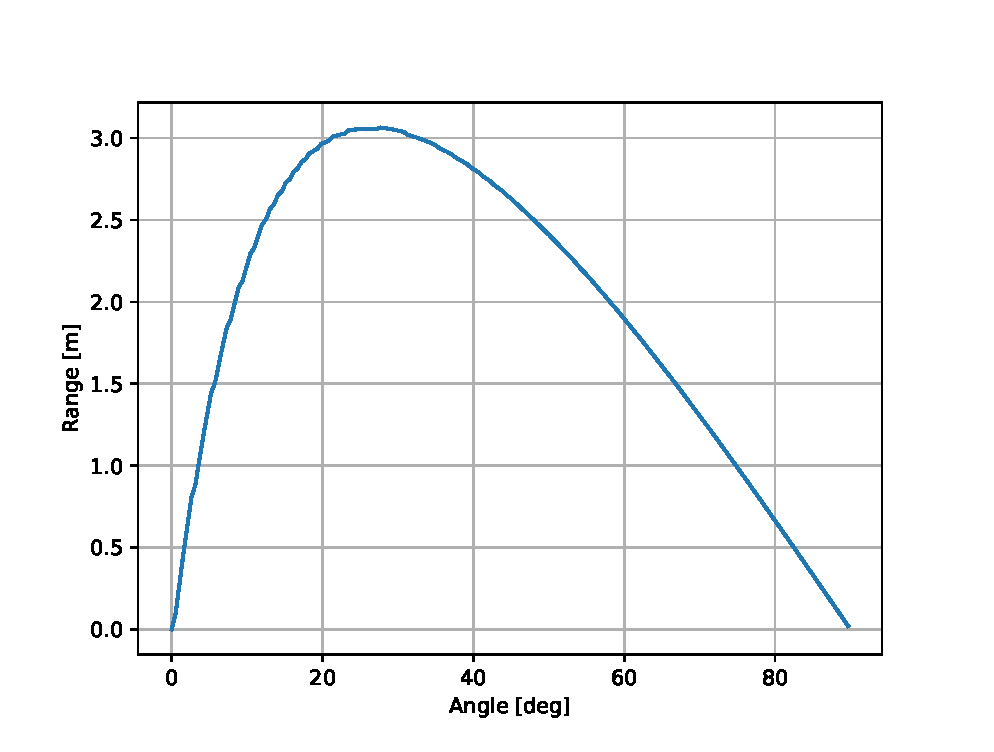
\includegraphics[width=0.9\textwidth]{ex3a.eps}
	\centering
	\caption{Συνάρτηση $R(\phi)$}
	\label{fig:ex3a}
	\includegraphics[width=0.9\textwidth]{ex3b.eps}
	\centering
	\caption{Τροχιά βλήματος για $\phi = \phi_{max}$}
	\label{fig:ex3b}
\end{figure}

Παρακάτω ακολουθεί ο κώδικας που γράφτηκε σε \textlatin{Python} και έγινε χρήση της βιβλιοθήκης \textlatin{Numpy}. Η υλοποίηση του αλγόριθμου \textlatin{Runge-Kutta} 4ης τάξης δίνεται στο Παράρτημα.
\selectlanguage{english}
\lstinputlisting[style=python, firstline=8]{ex3.py}
\end{document}